%# -*- coding: utf-8-unix -*-
% !TEX program = xelatex
% !TEX root = ../thesis.tex
% !TEX encoding = UTF-8 Unicode


\subsection{分阶段查询图生成}
\label{sec:compqa-candgen}
%TODO:先翻译,之后可以讲细一些,包括schema的定义,包括伪代码

本节中主要阐述分阶段候选查询图的生成过程。
与已有的工作比较,例如文献\parencite{bao2016constraint},
我们对候选生成的策略进行了优化,主要利用了查询图中对答案类型的隐含限制,
以及知识库中用来维护和时间段事实相关的特殊设计。
%The constraints that we can handle
本文中,我们主要考虑四种不同的语义限制,
分别是实体、类型、时间、顺序限制。
例如在问句中,实体限制描述了答案与某已知实体的联系,
顺序限制描述了答案按某种方式排序所具有的序号。
%我们更好地利用了知识库的类型信息,帮助过滤偏离查询图语义的类型限制,同时利用知识库对时间段事实的描述方式,
%(结果中配套显示我们的candgen结果高了多少,顺便还可以调整K画一些东西)
以\figref{fig:compqa-candgen}为例,
我们通过问句 ``who is the youngest president of the united states after 2002?''
阐述候选图的具体生成过程,该问句同时包含了上述四种语义限制。
为了方便描述,本节假设Freebase为问答系统所使用的知识库。

%  %it's a common practice to generate all possible query graphs through
%  %multiple stages~\cite{yih2015semantic,bao2016constraint}.
%  %Intuitively, the generation process begins from
%  %extracting candidate focus nodes in the question using linking tools.
%  %Then we connect the answer node to the corresponding focus entity
%  %using predicate sequences in KB.
%  %We call it ``main path'' and it is the basis of more complex structures.
%  %Further, we attempt to attach more constraints to the main path,
%  %%which are represented predicate sequences connect the remaining focus nodes to the main path,
%  %leading to complex query graphs in a tree shape.
%  %%The main intuition is to first find focus entities as the starting point of all candidate structures,
%  %%then extract main paths, and finally enrich the main path by adding different kinds of constraints.
%  We illustrate our staged candidate generation method in this section.
%  Compared to previous mathods, such as \citet{bao2016constraint}, we employ a more effective candidate
%  generation strategy, which takes advantage of implicit type information in query graphs
%  and time interval information in the KB.
%  In our work, we take 4 kinds of semantic constraints into account:
%  \textbf{entity}, \textbf{type}, \textbf{time} and \textbf{ordinal} constraints.
%  \figref{fig:candgen} shows a concrete example of our candidate generation.
%  For simplicity of discussion, we assume Freebase as the KB in this section.
%  %by performing SPARQL querys : generate main path first, and enrich add different kinds of constaints.


\begin{figure*}
	\centering
    \includegraphics[width=1\columnwidth]{figure/compqa/cangen.eps}
	\bicaption{分阶段候选图生成的具体例子。}{Running example of candidate generation.}
	\label{fig:compqa-candgen}
\end{figure*}


\textbf{阶段一:相关节点链接。}%(最好别叫相关实体,要区分focus和entity)
该步骤寻找问句中代表相关实体、类型、时间、顺序的词汇或短语,并链接到知识库上。
相关节点作为候选查询图的叶节点,是不同类别语义限制的起点。
\figref{fig:compqa-candgen}(a)列出了可能的\textless 短语,叶节点 \textgreater 对,
同一个短语可以对应到多个候选叶节点。
不同语义限制类别(实体、类型、时间、顺序)的叶节点有着各自的链接方式。
对于实体链接,我们使用了已有的链接工具S-MART\cite{yang2015s},
在多个已有的自动问答研究均被使用。
S-MART对所有可能的\textless 短语,实体 \textgreater 进行打分,并保留了至多前十组结果。
对于类型链接,考虑到知识库中不同的类型数量有限,
我们枚举问句中所有长度不超过3的短语,
并根据预训练的词向量,计算不同短语和类型之间的余弦相似度,
同样保留至多前十组结果。
对于时间链接,我们通过正则表达式识别句中出现的所有年份。
对于顺序链接,我们利用预先定义的形容词最高级词汇列表
(例如largest,highest,latest等描述客观事实的最高级词汇),
并在问句中匹配最高级词汇,或 ``{序数词+最高级}'' 的词组,如 ``second longest'' 。
对应的叶节点表示顺序值,若匹配到序数词,则顺序值为序数词对应的数字,否则为1。
如\figref{fig:compqa-candgen}(a)所示,\textless ``youngest'', 1 \textgreater
为生成的唯一顺序链接。

%  \textbf{Step 1: Focus linking.}
%  %This step takes the question as input, and returns candidate (mention, focus) pairs,
%  %where focus node 
%  %for example, (``United State'', \textit{united\_states})
%  We extract possible (mention, focus node) pairs from the question.
%  %We extract possible focus mentions (words or phrases in the question)
%  %and link them to nodes in KB or literal values.
%  Focus nodes are the starting points of various semantic constraints,
%  refer to \figref{fig:candgen}(a).
%  %for example in \figref{fig:candgen}(a),
%  %we link ``US'' to the entity \textit{united\_states},
%  %or ``US president'' to the type \textit{us\_president}.
%  %Different linking methods are used for different categories of focus nodes.
%  %For entity linking, we adopt a state-of-the-art linking tool, S-MART~\cite{yang2015s},
%  %which is widely used in previous KBQA researches.
%  %it scores candidate (mention, entity) pairs based on statistical features from Wikipedia,
%  %such as the lexical similarity, link probability and entity popularity.
%  %The output is a list of (mention, entity) with linking scores,
%  %and one mention can link to multiple entities.
%  For entity linking, we generate (mention, entity) pairs
%  using the state-of-the-art entity linking tool S-MART~\cite{yang2015s}.
%  %trained on Twitter corpus.
%  %Following the S-MART results provided by Yih et al.~\shortcite{yih2015},
%  %up to 10 top-ranked (mention, entity) pairs will be returned.
%  %One mention could lead to several entities.
%  %For example, the mention ``Star Trek'' links to several possible films in the result.
%  For type linking,
%  %due to the limited number of types in Freebase,
%  %we propose a simple but effective method for extracting (mention, type) pairs.
%  %we perform an embedding based brute force search.
%  we brutally combine each type with all uni-, bi- and tri-gram mentions in the question,
%  and pick top-10 (mention, type) pairs with the highest
%  word embedding similarities of each pair.
%  %we enumerate all uni-, bi- and tri-gram mentions of the question,
%  %and calculate the cosine similarities of averaging word embeddings
%  %between the mention and all the type names.
%  %Top-10 scoring (mention, type) pairs are kept as type linking results.
%  %and pair them with all the types in Freebase.
%  %For each (mention, type) pair, we calculate the cosine similarity
%  %of averaging word embedding vectors between them,
%  %and keep top-10 scoring pairs as type linking results.
%  For time linking, we extract time mentions by simply matching year regex.
%  For ordinal linking, we leverage a predefined superlative word list
%  \footnote{A list containing ~20 superlative words, such as largest, highest, latest.}
%  and recognize mentions by matching superlative words,
%  or the ``ordinal number + superlative'' pattern.
%  %``superlative'', ``ordinal number + superlative'' or ``superlative + adjective''.
%  The ordinal node is an integer representing the ordinal number in the mention.
%  %For example, we retrieve (``youngest'', 1) in \figref{fig:candgen}(a).



\textbf{阶段二:生成主路径。}
主路径是一个查询图的基础,代表着问句最主要的语义。
考虑到几乎所有的事实类问题都和问句中至少一个实体相关,
因此它被定义为从答案出发,通过谓词序列连接至某个实体节点的路径,
等同于一个简单问题的查询图。
我们枚举所有被链接的实体,以及它们在知识库中相连的合法谓词序列,
即可生成一系列候选主路径。
谓词序列的长度为1或2,后者实质是描述了多元关系中某两个实体的关联。
%通过知识库中的中间节点\footnote{Freebase中用于维护多元关系的辅助节点。}过渡。
\figref{fig:compqa-candgen}(b)显示出了某一个主路径,
其中答案节点$A$以及中间节点$v1$都是变量节点。%(是不是要多说几句?)
对于后续更复杂的语义限制,在图中均表示为由主路径上某变量节点出发,
指向特定的叶节点的谓词序列。

%  \textbf{Step 2: Main path generation.}
%  %We first build coarse query graphs by using focus entities only, since almost all factoid questions
%  %are related to at least one entity (except corner cases like ``Who's the fastest man in the world?'').
%  %The output of this step is refer to \figref{fig:candgen},
%  %where: one ore more entities are linked to the answer entity by FB predicates in a tree shape.
%  %For constructure different tree shapes,
%  We build different main paths by connecting the answer node to different focus entities
%  using 1-hop or 2-hop-with-mediator
%  %we first pick one focus entity and link the answer node to it by 1-hop or 2-hop-with-mediator
%  \footnote{Mediator is a kind of a auxiliary node in Freebase, used to maintain N-ary facts.}
%  predicate sequence.
%  \figref{fig:candgen}(b) shows one of the main paths.
%  Further constraints are attached by
%  %In the perspective of query graphs, a constraint is represented as a predicate sequence
%  connecting an anchor node $x$ to an unused focus node through predicate sequences,
%  where the anchor node $x$ is a non-focus node in the main path
%  ($A$ or $v_1$ in the example).
%  




\textbf{阶段三:添加额外实体语义限制。}
这个步骤的目的是在主路径之上扩充与实体相关的语义限制。
%所有出现的实体都可能会被用上
%深度搜索:
%枚举位置,连接位置,谓词,若有某种实例化方式,
%使得替代之后,均对应已存在的事实,则添加的限制有意义,引入新的实体,递归操作
受到\secref{sec:schema-candgen}中复杂模式图生成的启发,
我们同样采用深度优先搜索的方式,由简到繁进行查询图生成。
对搜索空间中的每一个查询图,我们尝试单个谓词连接不同的变量节点与实体节点,
构建出具有不同复杂程度的查询图。
如\figref{fig:compqa-candgen}(c)所示,在主路径上添加的
实体语义限制为($v_1, basic\_title, president$)。
基于深度优先搜索的优势在于查询图中的实体数量不受限,
和基于模板的候选生成方法相比,具有更高的覆盖率,
同时搜索过程中可以通过剪枝策略排除无法生成答案的查询图,提高候选生成速度。
%具体实现中,可以用SPARQL模糊查询,同时完成2-3步。
%可以考虑加伪代码,甚至聊SPARQL

%  \textbf{Step 3: Attaching entity constraints.}
%  %In this step, 
%  We apply a depth-first search to search for combinations of
%  multiple entity constraints to the main path through 1-hop predicate.
%  \figref{fig:candgen}(c) shows a valid entity constraint, ($v_1, basic\_title, president$).
%  The advantage of depth-first search is that we can involve unlimited number of entities
%  in a query graph, which has a better coverage than template-based methods.
%  %Fuzzy SPARQL queries are applied 
%  %for quickly finding all valid predicates between an anchor node and a focus entity,
%  %SPARQL query over Freebase all combination of predicates with certain shape.
%  
%  %Given all possible focus entitie of the question, we first build the main path of the query structure.
%  %We enumerate each entity as the main entity, and take the regard remaining as possible contraint entities.
%  %We search the knowledge base and explore all 1-hop and 2-hop-with-med predicate sequences
%  %starting from the main entity.
%  %For example, ...
%  %along this path, answer node could be xxxx and the intermediate entity are mediators describing the particular actor-film-starring fact.
%  %Afterwards, we attempt to add entity constraints to the main paths.
%  %%TODO: add SPARQL query example to the query structure
%  %if the constraint entity can be linked to the answer entity or intermediate entity by some 1-hop predicates.
%  %As the running example of Figure xxx, the constraint entity yyy is connected to the entity by the predicate "zzz".



\textbf{阶段四:添加类型限制。}
类型限制只能和答案节点关联,利用知识库中的\textit{IsA}谓词连接某个具体的相关类型节点。
在该步骤中,我们对已有方法进行了改进:通过答案节点直接连接的谓词,
推测出其具有的隐含类型,以此对类型限制进行过滤。
如\figref{fig:compqa-candgen}(c)所示,与答案直接相连的谓词为\textit{government\_position},
根据知识库对谓词的定义,其主语类型为\textit{politician},因此成为答案的隐含类型。
因此,我们可以过滤与隐含类型无关联的相关类型节点,
从而防止语义偏离,并提升候选差选图的生成速度。
具体而言,为了定义两个类型是否相关,我们采用了\secref{sec:tinf-approach-sort}中
通过松弛类型包含构建的Freebase类型层次关系。
若某相关类型不包含任意一个隐含类型,或不被任意一个隐含类型包含,
我们则将其视为无关类型,不用于候选生成。

% Our improvement in this step is to filter type constraints
% using \textbf{implicit types} of the answer, derived from the outgoing predicates 
% of the answer node.
% For example in \figref{fig:candgen}(c), 
% the domain type of the predicate \textit{government\_position}
% is \textit{politician}, which becomes the implicit type of the answer.
% Thus we can filter type constraints which are irrelevant to the implicit types,
% preventing semantic drift and speeding up the generation process.
% To judge whether two types in Freebase are relevant or not,
% we adopt the method in \citet{luo2015inferring} to build a rich type hierarchy of Freebase.
% Focus types are discarded, if they are not the super- or sub- types
% of any implicit types of the answer.

\textbf{阶段五:生成时间、顺序限制。}
完成类型限制的添加后,主路径上所有变量节点的类型(显式类型限制以及隐含类型)都已确定,
因此我们可以枚举隶属于这些类型的特定谓词,完成时间和顺序限制的添加。
如\figref{fig:compqa-candgen}(d)所示,时间限制通过长度为2的谓词序列表示,
例如序列[ \textit{from}, \textit{>} ],其中前一个谓词在知识库中指向时间,
后一个谓词为虚拟谓词,指明了和特定时间比较的方向,由问句中位于时间前的介词进行确定,
例如``before'', ``after'' 以及 ``in'' 。
类似地,顺序限制同样由长度为2的谓词序列表示,
例如序列[ \textit{date\_of\_birth}, \textit{MaxAtN} ],
前者在知识库中指向整数、浮点数或时间,后一个谓词表示降序排列。
我们并不能从问句中获取直接的信号确定排序方向\footnote{部分形容词最高级较为明显,
例如largest,longest等词几乎一定对应降序排列,但为了减少人工指定的规则,
我们不对这些形容词事先指定方向,而是通过模型训练进行学习。
},因此生成具体的排序限制时,两种方向都进行枚举。
值得注意的是,对于时间限制,我们的方法进行了针对性优化。
已有的文献\parencite{yih2015semantic,bao2016constraint}
仅考虑使用一条谓词与时间相连,
我们的改进在于使用了知识库中存在的\textbf{成对时间谓词},来描述更加准确的时间限制。
Freebase中,成对时间谓词用来描述和时间段相关的事实,
例如\figref{fig:compqa-candgen}(d)中的\textit{from}谓词,
存在谓词\textit{to}与之对应\footnote{$from$和$to$分别为
$government.government\_positions\_held.from$和
$government.government\_positions\_held.to$的简写。},
两者分别为起始时间谓词和终止时间谓词。
我们通过简单的名称匹配方式,收集了知识库中356组成对谓词,
对于时间比较为``in'' 的形式,例如句中出现``in 2002'' ,
我们在图中使用起始时间谓词进行连接,但生成SPARQL查询语句时,
起始和终止谓词均会被使用,从而确保问句中的相关时间能够限制在一个时间段内,
而不是仅仅等同于起始或终止时间点。

% As shown in \figref{fig:candgen}(d), the time constraint is represented
% as a 2-hop predicate sequence, 
% where the second is a virtual predicate determined by the preposition before the focus time,
% indicating the time comparing operation, like ``before'', ``after'' and ``in''.
% Similarly, the ordinal constraint also forms a 2-hop predicate sequence,
% where the second predicate represents descending (\textit{MaxAtN}) 
% or ascending order (\textit{MinAtN}).
% 
% For the detail of time constraint,
% while existing approaches \cite{yih2015semantic,bao2016constraint} 
% link the focus time with only single time predicate,
% our improvement is to leverage \textbf{paired time predicates}
% for representing a more accurate time constraint.
% %Suppose we are generating time constraints for the phrase ``in 2002'',
% In Freebase, paired time predicates are used to represent facts within certain time intervals,
% like $from$ and $to$\footnote{
% Short for $governmental\_position\_held.from$ and $governmental\_position\_held.to$
% respectively.} in \figref{fig:candgen}(d). 
% For time comparing operation ``in'', we link the time focus to the starting time predicate,
% but use both predicates in SPARQL query,
% restricting that the focus time lies in the time interval of the paired predicates.


所有阶段结束后,我们将所有生成查询图转换为SPARQL查询语句,并在Freebase中查询最终答案。
\figref{fig:compqa-candgen}(d)中的查询图对应的完整SPARQL查询语句\footnote{
$m.09c7w0$为实体``United States'' ,$m.060c4$为实体``President'' 。}对应如下:
\begin{lstlisting}[caption={SPARQL查询语句示例}]
PREFIX fb: <http://rdf.freebase.com/ns/>
SELECT ?ans ?name WHERE {
  ?ans fb:government.politician.government_positions_held ?v1 .
  ?v1 fb:government.government_position_held.jurisdiction_of_office fb:m.09c7w0 .
  ?v1 fb:government.government_position_held.basic_title fb:m.060c4 .
  ?v1 fb:government.government_position_held.from ?v3 .
  ?ans fb:type.object.type fb:government.us_president .
  ?ans fb:people.person.date_of_birth ?v2 .
  ?ans fb:type.object.name ?name .
  FILTER (?v3 >= "2002-01-01"^^xsd:dateTime) .
} ORDER BY DESC(?v2) LIMIT 1
\end{lstlisting}
最后,我们舍弃掉没有结果的查询图,以及使用的相关实体对应词组出现重叠的查询图。
和已有系统相比,本节的候选图生成使用了更少的人工规则,
并在类型限制和时间限制上进行了改进,加快生成速度的同时,描述更加准确的语义限制。

%  After finishing all these querying stages,
%  we translate candidate graphs into SPARQL query, producing their final output answers.
%  Finally, we discard query graphs with zero outputs, or using overlapped mentions.
%  %In summary, the candidate generation method is inspired by \citet{bao2016constraint},
%  %in summary, inspired by Yih, Bao: Fewer rules, and consider time interval.

